\documentclass[letterpaper]{article}

\usepackage[english]{babel}
\usepackage[utf8]{inputenc}
\usepackage{graphicx}
\usepackage{listings}
\usepackage[superscript,biblabel]{cite}
\usepackage[T1]{fontenc}

\title{Blocky: A Generalized Blockchain-Oriented Programming Language}

\author{Matthew Leeds (mwleeds@crimson.ua.edu)}

\date{November 23, 2015}

\begin{document}
\maketitle

\begin{abstract}
Ever since 2009 when Satoshi Nakamoto released the first workable blockchain-based application, Bitcoin, the technology has been an area of much interest, research, and development. While Bitcoin uses cryptographically linked ``blocks" of transactions to transfer money over the Internet, its decentralized consensus technology can be applied to a wide range of problems from censorship-resistant content hosting to trustless exchange systems. However there does not exist a common framework for the development of such apps with minimal effort on the developer's part and defined interoperability between them. Blocky seeks to fill this hole by providing a language for the creation of arbitrary blockchain-based applications.
\end{abstract}

\section{Introduction}

Bitcoin, Namecoin, Storj, and many other projects utilize very similar underlying cryptographic blockchains, each with unique application logic to serve the desired purpose (transfer money, register domain names, store files, etc). Because they each have separate blockchains, they each must convince users to run nodes in order to make the networks useful, and they must maintain a sizable code base to handle processing and propagation of blocks. If they could all be written in a well-defined common language, they could run on any compatible blockchain and thus would be much easier to develop and maintain.

The Ethereum project seeks to provide a blockchain, cryptocurrency, and language for deploying arbitrary blockchain apps, but its language (Solidity) only works in that system, whereas Blocky programs could be used on a variety of blockchains (whose cryptographic ciphers and transaction validation rules may differ) without changing their code. This can be accomplished because Blocky defines a set of interfaces that valid programs must implement as well as restrictions on usable language features to ensure well-behaved programs that can serve a wide range of potential purposes. Differences between Blocky and Solidity will be discussed further in a later section.

\section{The Blockchain Concept}
As implemented in the Bitcoin project, a blockchain is an append-only list of transactions in which later records are cryptographically linked to earlier ones in order to make modifying history computationally unfeasible. A symmetric key scheme is used to prove ownership over finite resources (such as bitcoins). Specifically, a user signs enough information to determine the origin and destination of the resource to be transferred using their private key.

\begin{figure}[h]
\centering
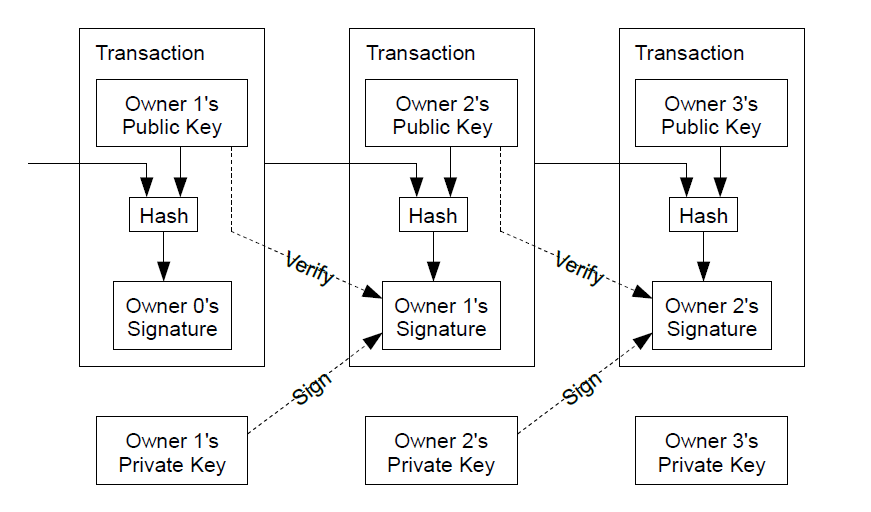
\includegraphics[width=0.7\textwidth]{transaction_chain.png}
\caption{\label{fig:transaction_chain}This is a simplified representation of transaction verification\cite{nakamoto09}.}
\end{figure}

This concept of transactions is generalized in Blocky so they can be used not just to transfer ``coins" (a special case of a finite, fungible resource) but to send messages to dapps that trigger operations.

In addition to verifying individual transactions, cryptography must again be used to arrive at decentralized consensus as to which transactions are considered valid and have been executed. The primary mechanism for this is including the hash of the previous block when determining the hash of each block. This way, modifying the historical record of transactions without changing the hash values requires either knowledge of a major vulnerability in the algorithm that's used or a prohibitive amount of computing power (for brute forcing).

\begin{figure}[h]
\centering
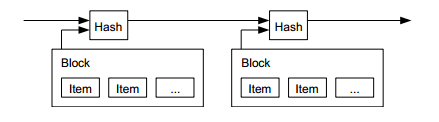
\includegraphics[width=0.7\textwidth]{blockchain.png}
\caption{\label{fig:blockchain}This is a high-level view of a blockchain\cite{nakamoto09}.}
\end{figure}

\section{Blocky's Execution Environment}

Blocky programs can execute on any computer running the software with a copy of the current blockchain. The host makes certain variables available to them, such as the current time and information about blockchain transactions. Transactions can either transfer money or call public methods (or you could view the former as a special case of the latter). The only ``side-effects" programs can have outside of their own stack variables is by broadcasting their own transactions to the network.

\section{Desirable Language Qualities}

The constraints and requirements of a blockchain ecosystem roughly dictate the following qualities that would maximize the usefulness of Blocky:
\begin{itemize}
  \item{Guaranteed termination or restricted computation time}
  \item{Turing completeness or as close as possible}
  \item{Access to relevant blockchain information}
  \item{No access to other resources on the host computer}
  \item{Definition of a standard interface for communication between dapps}
  \item{Familiarity for users of existing languages}
  \item{Generality to (almost) any blockchain}
\end{itemize}

The first and second points represent an unavoidable trade-off between arbitrary computation (Turing completeness) and guaranteed termination. Restricted computation time is important so that users cannot craft malicious or naive code that uses the computational resources of the host computer for an indefinite period of time. Unfortunately the only way to guarantee termination is to make the language less than Turing complete, meaning it will be impossible to implement certain classes of algorithms\cite{turing37}. Limiting the language's expressiveness also means the code can be more easily understood, both by humans and computers\cite{plant15}.

The third and fourth points regarding access to information are primarily security concerns. If peers could run truly arbitrary code on each other's computers, this would very quickly lead to OS vulnerabilities being exploited and clients could easily be compromised by malicious actors. But data access cannot be restricted entirely because programs must at least be able to send and receive information relevant to their activities in order for the system to be useful. By specifying well-defined interfaces for such messages, Blocky solves this problem.

If an interface for communication between program instances is defined by the language rather than individual projects, it will be more universal and therefore reduce unnecessary compatibility issues.

To reduce the learning curve and speed adoption, the language should feel familiar to users of popular languages, at least in its basic syntax, and ideally in its semantics to the extent possible. Blocky accomplishes this by staying close to the C\texttt{++} standard.

Blocky should be usable for as many blockchain systems as possible so that developers can reuse code and easily migrate between networks if such a need arises.

\section{Language Design and Specification}

Blocky is designed to share a significant amount of syntax and semantics with C\texttt{++}. Apart from providing familiarity, this makes it well-suited for efficient numerical computations, which are likely to be common (for example, cryptographic operations will occur frequently).

Similar to how classes are defined, \texttt{dapps} (decentralized applications) can be defined with public methods which are callable via transactions, and any number of private methods. A third classification for methods exists, \texttt{reusable}, which means those methods can be called by other dapps but execute in the context of the caller (whereas \texttt{public} methods execute in the context of the dapp that defined them). Here is the general layout of such a program (header file):
\begin{lstlisting}
dapp MyDapp {
  public:
    // constructor always takes 0 arguments
    MyDapp { type this.key = value; }
    
    @decorator
    type method(type param, ...);
    
  reusable:
    // methods that can be called by other dapps
    
  private:
    // possibly other helper functions
}
\end{lstlisting}
where \texttt{type} would be an actual data type. The \texttt{@decorator} can be either \texttt{@owner} or \texttt{@everyone}, which controls who can call the decorated method (using cryptographic authentication). While the owner is usually the original publisher, dapps can have more than one owner. Note the distinction between public/private and everyone/owner--- the former controls which cryptographically authenticated parties can execute code, whereas the latter is an enforcement of the author's intention of where the methods should be called (internally or externally to the dapp).

Syntax will be explained further in the examples below.

\subsection{Data Types}
Variables in Blocky are statically typed--- their types must be declared before they can be used. This system makes the code more explicit and readable, and protects against implicit variable declarations that may be accidental. Unlike C, Blocky uses strong typing so variables cannot be cast to other types and must be treated as their declared types. This can catch errors at compile-time in which the wrong variable is used in a statement. Further, numeric data types must explicitly declare their size in bytes (i.e. \texttt{int32\_t} or \texttt{int256\_t}, not just \texttt{int}). This rule makes potential for arithmetic overflow more obvious and forces code to execute comparably on different architectures (at least in this regard).

Static typing, strong typing, and explicit numeric types all lead to code that is more reliable, maintainable, and portable. 

\subsection{Scopes}
Here are the scopes of variables available to Blocky programs:
\begin{itemize}
  \item{variables in their own stack and key-value store}
  \item{variables defined by the host, such as the current time}
  \item{blockchain-level variables which include information about transactions}
\end{itemize}
Stack variables are only available for the duration of each execution. The key-value store provides persistent storage that can be modified via transactions. It is initialized at compile-time with the owner(s)' public key(s). Such values can be accessed using \texttt{this} since they are the dapp's only ``member" variables. Analogously, \texttt{host} and \texttt{chain} are used as prefixes to access variables in the other scopes mentioned. Of course the latter two scopes of variables are strictly read-only.

\subsection{Major Restrictions}
If any of the following conditions are broken, compilation will fail:
\begin{itemize}
  \item{\texttt{for} loops must have a deterministic invariant that will lead to termination.}
  \item{\texttt{GOTO}, \texttt{switch}, and \texttt{while} statements are not permitted.}
  \item{Code is not permitted to access anything outside its own data and that of the blockchain (filesystem, network, etc).}
\end{itemize}

\subsection{Comparison to Solidity}
As mentioned above, Ethereum is a project that aims to provide a blockchain to support the execution of smart contracts, which can be thought of as autonomous agents that can be programmed in a Turing-complete language, Solidity. Blocky seeks to solve roughly the same problem, but in a more general way. Here are the primary differences between the two languages:
\begin{itemize}
  \item{Blocky is more flexible as to what constitutes a valid transaction.}
  \item{Solidity code requires a virtual machine\cite{ethereum15}; Blocky code does not.}
  \item{Ethereum Virtual Machine instructions are restricted to 256-bit word operations\cite{ethereum15}. Blocky code can be compiled to any architecture.}
  \item{Addresses in Solidity are restricted to 160 bits\cite{ethereum15}. They can be any length in Blocky.}
  \item{Solidity contracts must use Ether\cite{ethereum15}. Blocky dapps can use any cryptocurrency.}
  \item{Library methods are integrated into Blocky dapps rather than being separate constructs.}
  \item{Function decorators are used to control access in Blocky, moving the responsibility of checking memory addresses from the dapp developer to the Blocky software.}
  \item{The caret notation for specifying maximum input size is unique to Blocky.}
\end{itemize}

\subsection{Compilation}
Steps taken by the Blocky compiler:
\begin{enumerate}
  \item{Remove comments and whitespace.}
  \item{Validate the syntax of the code (check brackets, semicolons, etc).}
  \item{Ensure that no side-effects are allowed outside of the dapp and blockchain.}
  \item{Do type checking.}
  \item{Do termination analysis to guarantee finite computation time (check \texttt{for} loop invariants, etc).}
  \item{Initialize the dapp's key-value store with the owner(s)' public key(s) and the dapp's address.}
  \item{Compile and dynamically link the code based on the blockchain addresses of dapps whose \texttt{public} or \texttt{reusable} methods are called.}
\end{enumerate}

Upon successful compilation, the user can publish their app into the blockchain using a transaction. Ideally there should be a way to produce deterministic builds so that users who compile from sources can check that their binary matches byte-for-byte with the official one for the same architecture, reducing the potential for malicious tampering.

\subsection{Built-in functions}
To make simple dapps possible without depending on \texttt{reusable} methods or re-implementing such things, Blocky provides common math functions (\texttt{power}, \texttt{sine}, \texttt{log}, etc) as well as standard cryptographic ciphers (\texttt{AES}, \texttt{SHA}, etc).

\textbf{Importantly, Blocky also provides the \texttt{transact(source, destination, key\_value\_store)} function for executing transactions on the blockchain from within dapps.} Such transactions are validated by the network which simply runs the dapp code and verifies that the provided inputs (from other transactions) produce the claimed transaction.

\subsection{Return values}
Unless otherwise specified, methods return a value of 0 of type \texttt{int8\_t} (signifying success).

\section{Examples}

Some examples of decentralized apps that could be built using Blocky:
\begin{itemize}
  \item{A minimal-overhead, market-based cryptocurrency exchange}
  \item{A trustless exchange system for real-world goods and services (assuming there exists a reliable out-of-band way to verify receipt of such goods)}
  \item{A trustless crowdfunding platform}
  \item{A censorship-resistant content hosting platform}
  \item{An encrypted, redundant storage network}
  \item{A fully democratically run corporation}
  \item{A provably fair gambling system}
  \item{Time-dependent transactions}
\end{itemize}
\bigskip
Let's look at code for some of these.
\subsection{A Gambling System}
\begin{lstlisting}
dapp Gambler {
  public:
    Gambler { uint64_t this.balance = 0; }
    
    @owner
    withdraw_balance() { // the owner can withdraw at any time
      if (this.balance > 0)
        transact(this.addr, this.owner, {"amount": this.balance});
    }
    
    @everyone
    int8_t gamble(uint256_t better, uint32_t amount) {
      if (chain.block_hash % host.time == 0) { // winner takes all
        transact(this.addr, better, {"amount": this.balance});
        return 0;
      } else {
        // the contract collects the bet
        transact(better, this.addr, {"amount": amount});
        this.balance += amount;
        return 1;
      }
    }
}
\end{lstlisting}
This simple gambling system relies on the current time and the current's block's hash value for unknowable entropy (the hash is determined until the transaction is included in a block), and given that it's likely extremely improbable that the block hash will be perfectly divisible by the current time, it seems only fair that the better should receive all the available money.
\newline

\subsection{Delayed Purchasing}
\begin{lstlisting}
dapp DelayedPurchase {
  public:
    @owner
    int8_t buy_if_past_date() {
      if (host.time > 1448344800) { // using UNIX time
        // buy something using a hardcoded dapp address
        transact(this.addr, 0x809FBDA8, {"amount": 42});
        return 0;
      } else {
        return 1;
      }
    }
}
\end{lstlisting}
As you can see, this dapp ensures that a purchase will occur at a certain date (or at least no earlier). One interesting application for this type of code could be leaving money to your descendants but not releasing it until they reach a certain age (without having to pay a lawyer).
\newline

\subsection{Simple Content Hosting}
\begin{lstlisting}
dapp ContentHost {
  public:
    ContentHost { string -> bytes[^1024] storage = []; }
    
    @owner
    put_content(string key, bytes[^1024] value) {
      this.storage[key] = value;
    }
    
    @everyone
    bytes[] get_content(string key) {
      if (key in this.storage)
        return this.storage[key];
      else
        return [];
    }
}
\end{lstlisting}
In the code above, the caret before 1024 is a way to specify a maximum input size. This requirement is enforced by transaction validation code on clients.
\newline

\subsection{Trustless Crowdfunding}
\begin{lstlisting}
dapp Crowdfund {
  public:
    Crowdfund {
      uint16_t this.funding_goal = 4200;
      uint16_t this.balance = 0;
      // here is the syntax for defining a mapping
      uint16_t -> uint16_t this.funders = [];
    }
    
    @owner
    int8_t release_money() {
      if (this.balance >= this.funding_goal) {
        // crowdfunding succeeded, start the project
        transact(this.addr, this.owner, this.balance);
        return 0;
      } else {
        // crowdfunding did not reach the goal; return the money
        for (uint16_t contributor in this.funders) { // implicit iterator
          transact(this.addr, contributor, this.funders[contributor]);
        }
        return 1;
      }
    }
    
    @everyone
    contribute(uint256_t src, uint16_t amount) {
      transact(src, this.addr, amount);
      this.balance += amount;
      this.funders[src] = amount;
    }
}
\end{lstlisting}
This code collects money from people who want to kickstart a project, and, once prompted by the owner, releases it to the project or sends it all back, depending on whether the funding goal was reached. A mechanism could trivially be added to enforce a deadline as well.
\newline

\subsection{A Democratic Corporation}
\begin{lstlisting}
dapp DemCorp {
  public:
    DemCorp {
      // map reusable methods to the votes accumulated for them
      uint256_t -> uint16_t this.motions = [];
      // require 2/3 agreement for action on something
      uint16_t this.action_threshold = 0.66 * this.owners.length;
    }
    
    @owner // this includes all shareholders
    vote_for_motion(uint256_t motion) {
      if (motion not in this.motions)
        this.motions[motion] = 0;
      else
        this.motions[motion]++;
      if (this.motions[motion] >= this.action_threshold) {
        // consensus was reached; take action
        transact(this.addr, motion, {});
      }
    }
    
    @owner
    add_owner(uint256_t new_owner) {
      if (new_owner not in this.owner)
        this.owner.append(new_owner);
    }
    
    @owner
    remove_owner(uint256_t existing_owner) {
      if (existing_owner in this.owner)
        this.owner.remove(existing_owner);
    }
}
\end{lstlisting}
This code allows shareholders to have equal votes in controlling the actions of a corporation. In the simplest case, the dapp controls an external organization but the fully decentralized model would be for the dapp to \textit{be} the organization. Mechanisms could be implemented to require a certain quorum of owners for action, or to have a different threshold for more important decisions (such as changing the threshold itself).
\newline

\subsection{A Short Library}
\begin{lstlisting}
dapp BlockchainLib {
  reusable:
    // remember the following methods execute in the caller's context
    int512_t getBalance() {
      // balance can only become negative during calculation
      int512_t balance = 0;
      for (block_type block in chain.blocks) {
        for (tx_type transaction in block) {
          if (transaction.from == this.addr)
            balance -= transaction.amount;
          if (transaction.to == this.addr)
            balance += transaction.amount;
        }
      }
      return balance;
    }
}
\end{lstlisting}
Of course production-quality libraries are likely to be longer and more robust, but this provides a simple example of a reusable function that uses the blockchain and its calling dapp's address to calculate a balance.
\newline

\section{Potential Improvements}
To afford scalability, a mechanism could be provided so programs would only need to be executed on a subset of participating nodes, rather than the entire network. Similarly, a mechanism for parallelizing code would help Blocky make more efficient use of available resources.

Another potential improvement would be to provide more fine-grained control over method access than just \texttt{@owner} and \texttt{@everyone}.
\begin{thebibliography}{9}

\bibitem{nakamoto09}
  Satoshi Nakamoto,
  ``Bitcoin: A Peer-to-Peer Electronic Cash System",
  http://bitcoin.org/bitcoin.pdf
  
\bibitem{turing37}
  Alan Turing,
  ``On Computable Numbers, With an Application to the Entscheidungs Problem",
  Proc. London Math. Soc. (1937) s2-42 (1): 230-265.
  doi: 10.1112/plms/s2-42.1.230.
  
\bibitem{plant15}
  Luke Plant,
  ``We Need Less Powerful Languages",
  Published 14 November 2015.
  http://lukeplant.me.uk/blog/posts/less-powerful-languages/.
  
\bibitem{ethereum15}
  Solidity Documentation
  https://ethereum.github.io/solidity/docs/home/

\end{thebibliography}
  
\end{document}
